
	\chapter{RESULTS \& DISCUSSION}
	\label{chap:results}
	
	\section{Tabulations}
	
		\begin{table}[]
			\caption{Most Economic Time interval to Charge the Vehicle}
			\centering
		\begin{tabular}{|l|l|l|l|}
			\hline
			\textbf{VEHICLE TYPE}           & \textbf{CASE}         & \textbf{BEST PRICE} & \textbf{HOUR} \\ \hline
			\multirow{3}{*}{\textbf{CAR}}   & \textbf{Case 1 - (00:00)} & - \$1.71            & 12:00         \\ \cline{2-4} 
			& \textbf{Case 2 - (00:20)} & - \$2.09            & 01:20         \\ \cline{2-4} 
			& \textbf{Case 3 - (00:40)} & - \$1.58            & 01:40         \\ \hline
			\multirow{3}{*}{\textbf{BUS}}   & \textbf{Case 1 - (00:00)} & - \$0.47            & 12:00         \\ \cline{2-4} 
			& \textbf{Case 2 - (00:20)} & - \$1.25            & 20:20         \\ \cline{2-4} 
			& \textbf{Case 3 - (00:40)} & - \$0.69            & 11:40         \\ \hline
			\multirow{3}{*}{\textbf{TRUCK}} & \textbf{Case 1 - (00:00)} & - \$2.57            & 05:00         \\ \cline{2-4} 
			& \textbf{Case 2 - (00:20)} & -\$1.00             & 04:20         \\ \cline{2-4} 
			& \textbf{Case 3 - (00:40)} & - \$2.11            & 04:40         \\ \hline
		\end{tabular}
	\end{table}



\begin{table}[]
	\centering
	\caption{Power Loss when Ev connected in different busses in 33 bus system for two load profile scenarios}
	\begin{tabular}{|c|c|cc|cc|cc|}
		\hline
		\multirow{2}{*}{\textbf{Scenario}}                            & \multirow{2}{*}{\textbf{\begin{tabular}[c]{@{}c@{}}Base\\ Case\\ Power\\ Loss\end{tabular}}} & \multicolumn{2}{c|}{\textbf{Case 1}}                                                                                                                                                                          & \multicolumn{2}{c|}{\textbf{Case 2}}                                                                                                                                                                          & \multicolumn{2}{c|}{\textbf{Case 3}}                                                                                                                                                                          \\ \cline{3-8} 
		&                                                                                              & \multicolumn{1}{c|}{\textbf{\begin{tabular}[c]{@{}c@{}}Power \\ Loss\\ when EV\\ in Bus 2\\ (kW)\end{tabular}}} & \textbf{\begin{tabular}[c]{@{}c@{}}Power \\ Loss\\ when EV\\ in Bus 18\\ (kW)\end{tabular}} & \multicolumn{1}{c|}{\textbf{\begin{tabular}[c]{@{}c@{}}Power \\ Loss\\ when EV\\ in Bus 2\\ (kW)\end{tabular}}} & \textbf{\begin{tabular}[c]{@{}c@{}}Power \\ Loss\\ when EV\\ in Bus 18\\ (kW)\end{tabular}} & \multicolumn{1}{c|}{\textbf{\begin{tabular}[c]{@{}c@{}}Power\\  Loss\\ when EV\\ in Bus 2\\ (kW)\end{tabular}}} & \textbf{\begin{tabular}[c]{@{}c@{}}Power \\ Loss\\ when EV\\ in Bus 18\\ (kW)\end{tabular}} \\ \hline
		\textbf{\begin{tabular}[c]{@{}c@{}}Scenario\\ 1\end{tabular}} & \multirow{2}{*}{202.691}                                                                     & \multicolumn{1}{c|}{204.104}                                                                                    & 253.746                                                                                     & \multicolumn{1}{c|}{65.773}                                                                                     & 78.460                                                                                      & \multicolumn{1}{c|}{204.104}                                                                                    & 253.746                                                                                     \\ \cline{1-1} \cline{3-8} 
		\textbf{\begin{tabular}[c]{@{}c@{}}Scenario\\ 2\end{tabular}} &                                                                                              & \multicolumn{1}{c|}{189.833}                                                                                    & 236.912                                                                                     & \multicolumn{1}{c|}{178.967}                                                                                    & 222.468                                                                                     & \multicolumn{1}{c|}{189.833}                                                                                    & 236.912                                                                                     \\ \hline
	\end{tabular}
				\label{table:powerloss}
\end{table}




	\begin{table}[h]
		\centering
		\caption{Hour at which the EV Load is maximum }
		\begin{tabular}{|ll|ll|ll|ll|}
			\hline
			\multicolumn{2}{|l|}{\textbf{SCENARIO}} & \multicolumn{2}{l|}{\textbf{HOURLY}} & \multicolumn{2}{l|}{\textbf{20MINS}} & \multicolumn{2}{l|}{\textbf{40 MINS}} \\ \hline
			\multicolumn{2}{|l|}{\textbf{SCENARIO-1}}        & \multicolumn{2}{l|}{$ 13^{th} $}            & \multicolumn{2}{l|}{$ 6^{th} $}             & \multicolumn{2}{l|}{$ 13^{th} $}             \\ \hline
			\multicolumn{2}{|l|}{\textbf{SCENARIO-2}}        & \multicolumn{2}{l|}{$ 19^{th} $}           & \multicolumn{2}{l|}{$ 6^{th} $}             & \multicolumn{2}{l|}{$ 19^{th} $}             \\ \hline
		\end{tabular}
	\end{table}
		
		
		
		
		
		
		
	\section{Charging Patterns}
			\begin{figure}
				\centering
				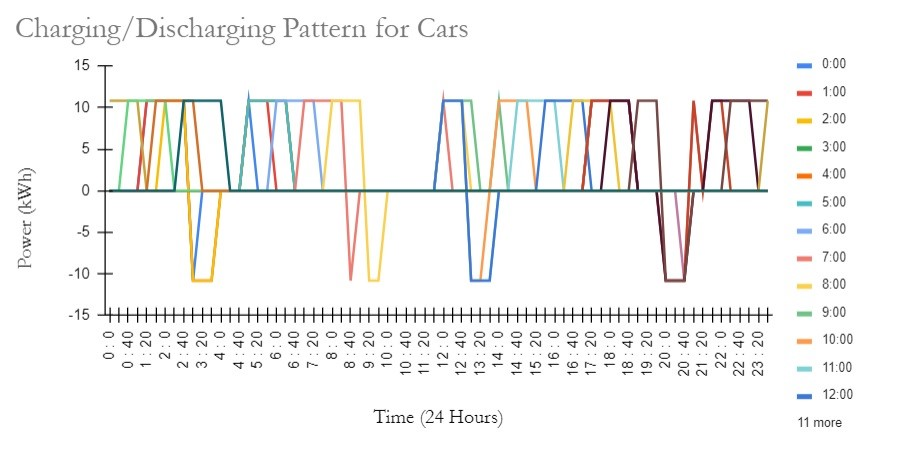
\includegraphics[width=0.7\linewidth]{C:/Users/HP/Downloads/cp_case1}
				\caption{}
				\label{fig:cpcase1}
			\end{figure}
			\begin{figure}
				\centering
				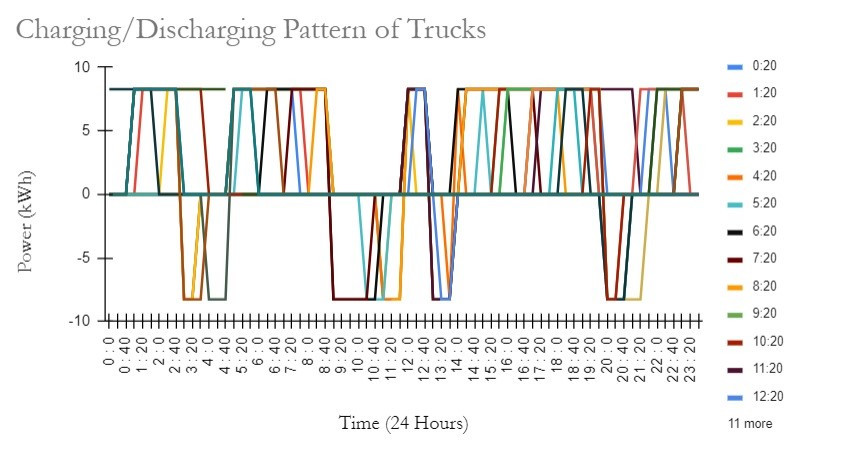
\includegraphics[width=0.7\linewidth]{C:/Users/HP/Downloads/cp_case2}
				\caption{}
				\label{fig:cpcase2}
			\end{figure}
		
			\begin{figure}
				\centering
				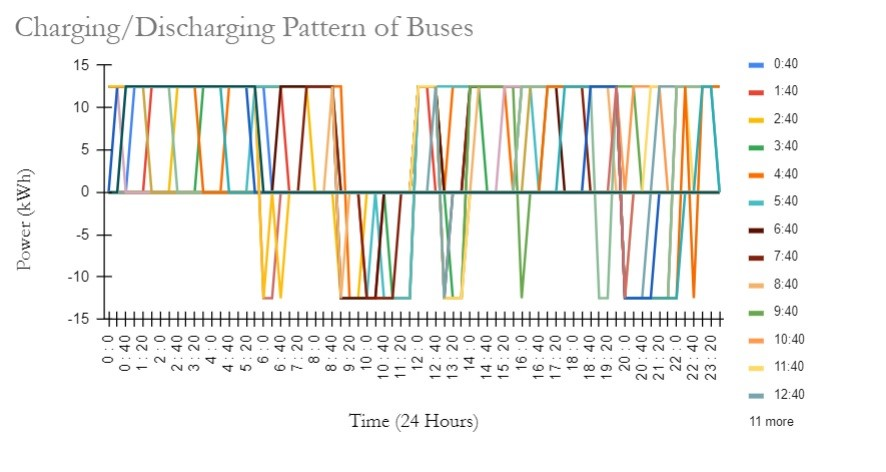
\includegraphics[width=0.7\linewidth]{C:/Users/HP/Downloads/cp_case3}
				\caption{}
				\label{fig:cpcase3}
			\end{figure}
			
			
			
			
			
			
			
	\section{Voltage Magnitude Graphs for Different Scenarios}
	
	 \begin{figure}[!h]
		\begin{subfigure}{.5\textwidth}
			\centering
			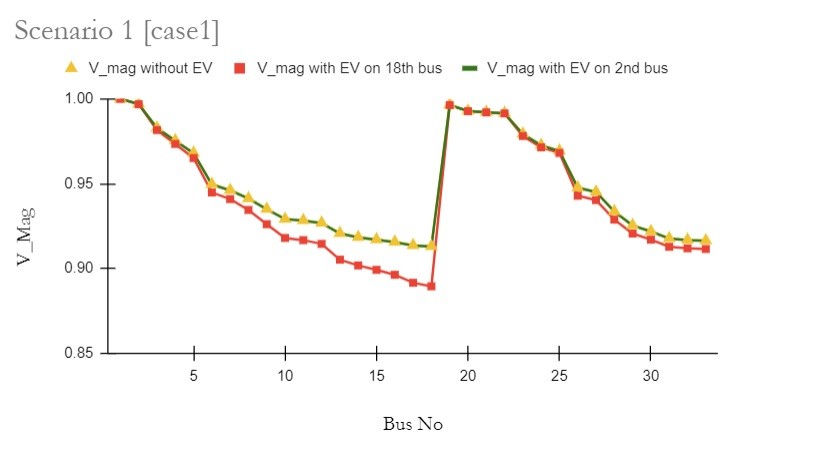
\includegraphics[width=.97\linewidth,height= 4.95cm]{./Figures/sc1_case1}  
			\caption{Case I}
			\label{fig:LFa}
		\end{subfigure}
		\begin{subfigure}{.5\textwidth}
			\centering
			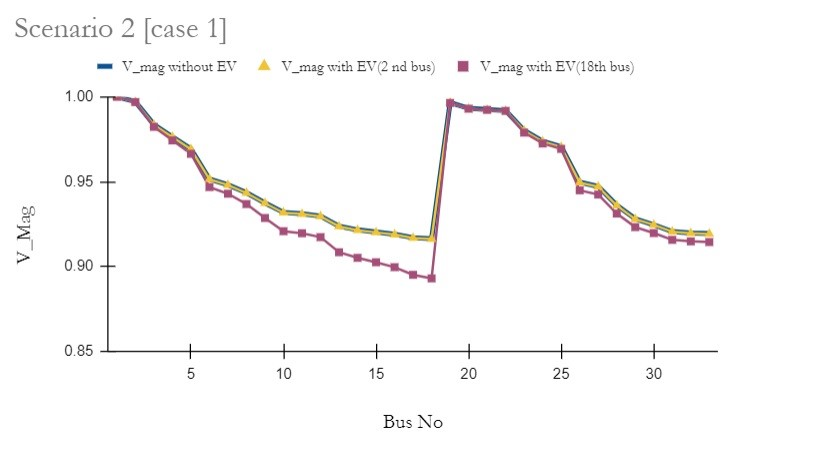
\includegraphics[width=.97\linewidth,height= 4.95cm]{./Figures/sc2_case1}  
			\caption{Case I}
			\label{fig:LF2a}
		\end{subfigure}
		\begin{subfigure}{.5\textwidth}
			\centering
			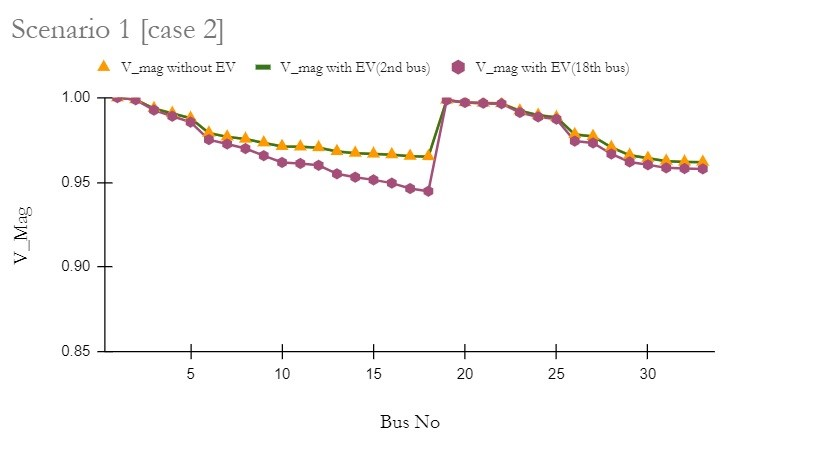
\includegraphics[width=.97\linewidth,height= 4.95cm]{./Figures/sc1_case2}
			\caption{Case II}
			\label{fig:LFb}
		\end{subfigure}
		\begin{subfigure}{.5\textwidth}
			\centering
			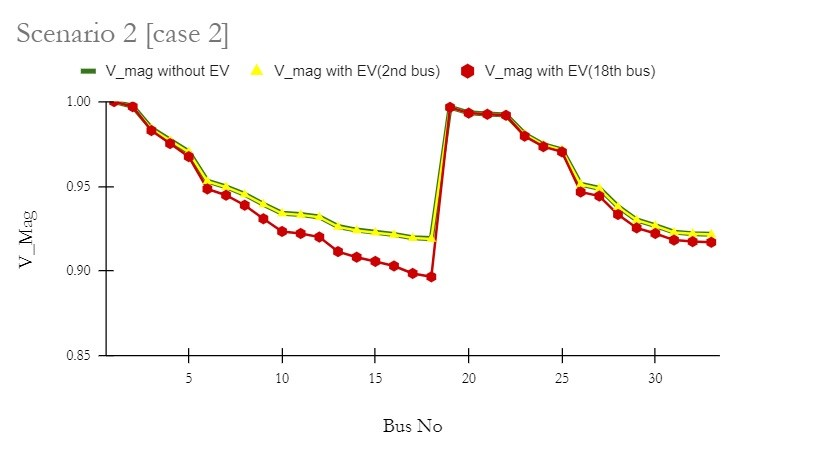
\includegraphics[width=.97\linewidth,height= 4.95cm]{./Figures/sc2_case2}
			\caption{Case II}
			\label{fig:LF2b}
		\end{subfigure}
		\begin{subfigure}{.5\textwidth}
			\centering
			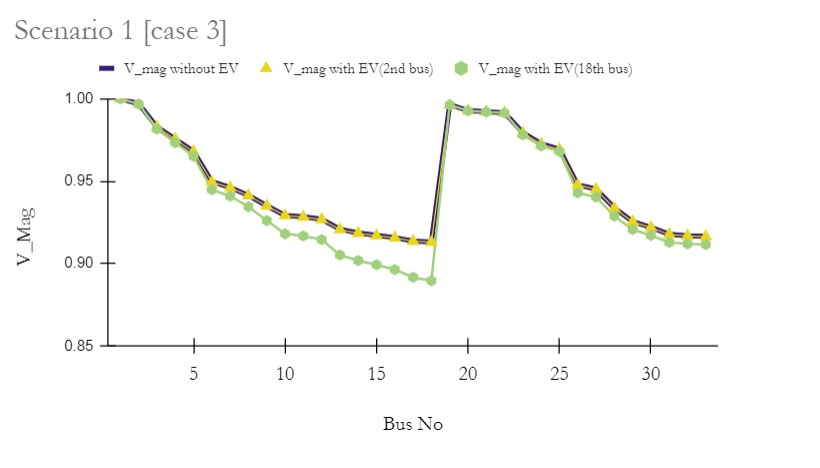
\includegraphics[width=.97\linewidth,height= 4.95cm]{./Figures/sc1_case3}
			\caption{Case III}
			\label{fig:LFc}
		\end{subfigure}
		\begin{subfigure}{.5\textwidth}
			\centering
			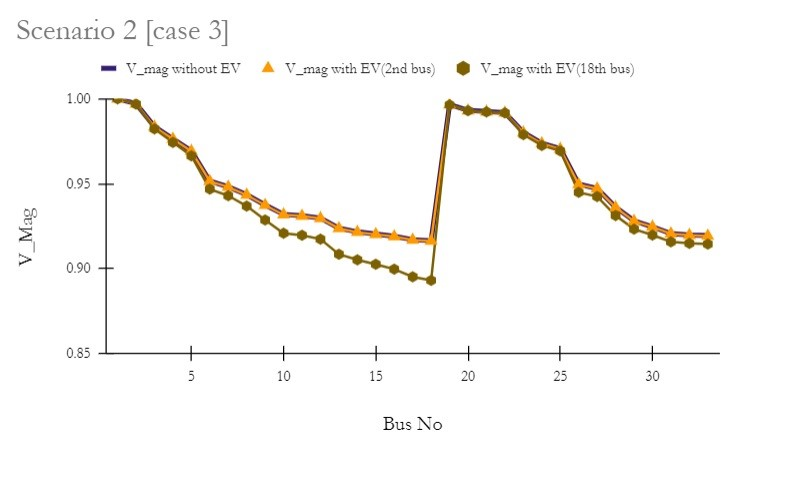
\includegraphics[width=.97\linewidth,height= 4.95cm]{./Figures/sc2_case3}
			\caption{Case III}
			\label{fig:LF2c}
		\end{subfigure}
		\caption{ Voltage magnitude variation for different scenarios }
		\label{fig:loadprofile-scenario1}
	\end{figure} 
	
	


		
	
	
	